\documentclass[12pt,a4paper]{article}

% ─── Page Layout ───────────────────────────────────────────────────────────────
\usepackage[a4paper, margin=0.8in, headheight=14pt]{geometry}

% ─── Fonts (XeLaTeX) ───────────────────────────────────────────────────────────
\usepackage{fontspec}
\usepackage{unicode-math}
\setmainfont{TeX Gyre Pagella}
\setmonofont[Scale=0.88]{TeX Gyre Cursor}
\setmathfont{Latin Modern Math}

% ─── Packages ──────────────────────────────────────────────────────────────────
\usepackage{xcolor}
\usepackage{colortbl}
\usepackage{titlesec}
\usepackage{enumitem}
\usepackage{tabularx}
\usepackage{booktabs}
\usepackage{array}
\usepackage{amsmath}
\usepackage{tikz}
\usetikzlibrary{shapes.geometric, arrows.meta, positioning, calc, fit, decorations.pathreplacing, patterns}
\usepackage{tcolorbox}
\tcbuselibrary{skins, breakable}
\usepackage{hyperref}
\usepackage{fancyhdr}
\usepackage{graphicx}
\usepackage{microtype}
\hyphenpenalty=10000
\exhyphenpenalty=10000
\sloppy
\usepackage{caption}
\usepackage{setspace}
\usepackage{multirow}
\usepackage{tocloft}

% ─── Q&A helper ────────────────────────────────────────────────────────────────
\newcommand{\Q}[1]{\textbf{#1}\par\noindent\ignorespaces}

% ─── Colour Palette ────────────────────────────────────────────────────────────
\definecolor{myred}{RGB}{196,30,58}
\definecolor{mydark}{RGB}{30,30,50}
\definecolor{mygreen}{RGB}{14,120,80}
\definecolor{myteal}{RGB}{0,130,140}
\definecolor{myamber}{RGB}{180,100,0}
\definecolor{mypurple}{RGB}{100,30,160}
\definecolor{mygray}{RGB}{246,247,249}
\definecolor{mgframe}{RGB}{180,185,200}
\definecolor{watermark}{RGB}{145,150,170}
\definecolor{hdrred}{RGB}{250,232,235}
\definecolor{hdrgreen}{RGB}{220,244,233}
\definecolor{hdrteal}{RGB}{220,242,244}
\definecolor{hdramber}{RGB}{253,242,215}
\definecolor{hdrpurple}{RGB}{238,228,255}
\definecolor{hdrgray}{RGB}{238,240,245}
\definecolor{rowalt}{RGB}{250,251,253}

% ─── Section Formatting ────────────────────────────────────────────────────────
\titleformat{\section}{\large\bfseries\color{myred}}{\thesection.}{0.5em}{}[\vspace{1pt}{\color{myred}\rule{\linewidth}{0.8pt}}]
\titleformat{\subsection}{\normalsize\bfseries\color{myteal}}{\thesubsection}{0.5em}{}
\titlespacing*{\section}{0pt}{18pt}{7pt}
\titlespacing*{\subsection}{0pt}{11pt}{4pt}

% ─── Paragraph ─────────────────────────────────────────────────────────────────
\setlength{\parindent}{0pt}
\setlength{\parskip}{4pt}

% ─── TOC Styling ───────────────────────────────────────────────────────────────
\renewcommand{\cfttoctitlefont}{\large\bfseries\color{myred}}
\renewcommand{\cftaftertoctitle}{\par\noindent{\color{myred}\rule{\linewidth}{0.8pt}}}
\setlength{\cftbeforetoctitleskip}{0pt}
\setlength{\cftaftertoctitleskip}{6pt}
\renewcommand{\cftsecfont}{\normalsize\bfseries\color{mydark}}
\renewcommand{\cftsecpagefont}{\normalsize\bfseries\color{mydark}}
\renewcommand{\cftsecleader}{\cftdotfill{\cftdotsep}}
\setlength{\cftbeforesecskip}{7pt}
\renewcommand{\cftsubsecfont}{\small\color{mydark}}
\renewcommand{\cftsubsecpagefont}{\small\color{mydark}}
\setlength{\cftbeforesubsecskip}{3pt}
\setlength{\cftsubsecindent}{1.4em}

% ─── Table helpers ─────────────────────────────────────────────────────────────
\renewcommand{\arraystretch}{1.45}
\setlength{\tabcolsep}{6pt}
\arrayrulecolor{mydark}
\newcolumntype{B}[1]{>{\small\bfseries\raggedright\arraybackslash}m{#1}}
\newcolumntype{Y}{>{\small\raggedright\arraybackslash}X}
\renewcommand{\tabularxcolumn}[1]{m{#1}}

% ─── Header / Footer ───────────────────────────────────────────────────────────
\pagestyle{fancy}
\fancyhf{}
\fancyhead[L]{\small\color{myred}\textbf{OE-EC803A}\;\color{mydark}--- Internet of Things}
\fancyhead[R]{\small\color{myteal}\textbf{Module 6 Notes}}
\fancyfoot[C]{\small\color{mydark}\thepage}
\fancyfoot[R]{\small\color{watermark}\textit{\copyright\ Biraj Sarkar}}
\renewcommand{\headrulewidth}{0.5pt}
\renewcommand{\footrulewidth}{0.3pt}

% ─── Hyperref ──────────────────────────────────────────────────────────────────
\hypersetup{colorlinks=true, linkcolor=myteal, urlcolor=myteal,
  pdfauthor={Biraj Sarkar}, pdftitle={OE-EC803A --- Module 6 Notes}}

% ─── tcolorbox styles ──────────────────────────────────────────────────────────
\tcbset{
  tikzbox/.style={colback=mygray, colframe=mgframe, boxrule=0.6pt, arc=4pt,
    left=8pt, right=8pt, top=6pt, bottom=6pt,
    colbacktitle=mgframe, coltitle=mydark, fonttitle=\small\bfseries},
  defbox/.style={colback=hdrgreen, colframe=mygreen, boxrule=0.8pt, arc=4pt,
    left=9pt, right=9pt, top=6pt, bottom=6pt,
    colbacktitle=mygreen, coltitle=white, fonttitle=\small\bfseries},
  formulabox/.style={colback=hdrteal, colframe=myteal, boxrule=0.8pt, arc=4pt,
    left=9pt, right=9pt, top=7pt, bottom=7pt,
    colbacktitle=myteal, coltitle=white, fonttitle=\small\bfseries},
  examplebox/.style={colback=hdramber, colframe=myamber, boxrule=0.8pt, arc=4pt,
    left=9pt, right=9pt, top=6pt, bottom=6pt,
    colbacktitle=myamber, coltitle=white, fonttitle=\small\bfseries},
  masonbox/.style={colback=hdrpurple, colframe=mypurple, boxrule=0.8pt, arc=4pt,
    left=9pt, right=9pt, top=6pt, bottom=6pt,
    colbacktitle=mypurple, coltitle=white, fonttitle=\small\bfseries},
  exambox/.style={colback=hdrpurple, colframe=mypurple, boxrule=1pt, arc=5pt,
    left=10pt, right=10pt, top=8pt, bottom=8pt,
    colbacktitle=mypurple, coltitle=white, fonttitle=\bfseries,
    breakable, title after break={\textbf{Frequently Asked / Viva Questions (contd.)}}}
}
\tcbset{breakable}

% ─── TikZ styles ───────────────────────────────────────────────────────────────
\tikzset{
  block/.style={rectangle, draw=myteal, fill=hdrteal,
    text width=2.2cm, align=center, minimum height=0.85cm,
    font=\small, rounded corners=3pt, line width=0.7pt},
  arrow/.style={-Stealth, thick, color=mydark},
  line/.style={draw, thick, color=mydark}
}

\begin{document}

% ═══════════════════════════════════════════════════════════════════════════════
% TITLE BLOCK
% ═══════════════════════════════════════════════════════════════════════════════
\begin{center}
  \hfill \textit{Exam-Ready Short Notes} \\
  \vspace{6pt}
  {\LARGE\bfseries\color{myred} OE-EC803A --- Internet of Things}\\[5pt]
  {\normalsize\color{mydark} Semester VIII \quad$\bullet$\quad 3L:0T:0P \quad$\bullet$\quad 3 Credits}\\[3pt]
  {\normalsize\color{myteal}\textbf{Module 6: Prototype to Reality: Business, Manufacturing \& Ethics}}\\[3pt]
  {\small\color{mydark} CGEC \;$|$\; B.Tech ECE (2023--27) \;$|$\; \textit{Biraj Sarkar}}
\end{center}
\vspace{2pt}
\noindent{\color{myred}\rule{\linewidth}{1.5pt}}
\vspace{2pt}

\hypersetup{linkcolor=mydark}
\tableofcontents
\hypersetup{linkcolor=myteal}
\newpage

% ===============================================================================
\section{IoT Business Models \& Startups}
% ===============================================================================

Transitioning an IoT prototype into a commercial product requires establishing sustainable business value.

\subsection{A Short History of Business Models}
Historically, business models revolved around the \textbf{transactional model} (Value-Transaction-Exchange), where companies designed, manufactured, and sold physical products as a one-time purchase. 
In the digital age, this evolved into the \textbf{subscription/service-based model} (e.g. SaaS). IoT merges these two histories: it combines the transactional sale of physical hardware with the ongoing subscription-based service model (Product-as-a-Service), creating a continuous customer relationship.

\subsection{Who is the Business Model For?}
An IoT business model serves three main target audiences:
\begin{itemize}[leftmargin=*, itemsep=3.0pt]
  \item \textbf{Investors:} Demonstrates the viability, return on investment (ROI), scalability, and path to profitability (amortizing high upfront tooling and NRE costs).
  \item \textbf{Partners and Suppliers:} Clarifies roles in the value chain, such as PCB manufacturing houses, cloud providers, and distribution networks.
  \item \textbf{Internal Team:} Aligns the engineering, sales, and support departments on customer needs, product value propositions, and resource allocations.
\end{itemize}

\subsection{Business Model Canvas in IoT}
The \textbf{Business Model Canvas} defines a startup's value chain across 9 building blocks. IoT products alter these blocks:
\begin{enumerate}[leftmargin=*, itemsep=3.0pt]
  \item \textbf{Value Proposition:} Continuous software updates, predictive maintenance, and remote automation rather than just static physical utility.
  \item \textbf{Revenue Streams:} Low upfront hardware margins compensated by recurring subscription models (SaaS / Hardware-as-a-Service).
  \item \textbf{Customer Segments:} Distinct B2C (consumers desiring convenience) vs. B2B (enterprises desiring efficiency/analytics).
  \item \textbf{Customer Relationships:} Continuous digital engagement via apps and automated support, rather than one-time transaction endpoints.
  \item \textbf{Channels:} Digital app stores and direct e-commerce, paired with physical retail and distribution channels.
  \item \textbf{Key Activities:} Firmware maintenance, OTA software updates, security patch deployment, and cloud server scaling.
  \item \textbf{Key Resources:} Proprietary sensor algorithms, cloud database infrastructure, engineering talent, and manufacturing supply chains.
  \item \textbf{Key Partners:} Cloud platform providers (AWS, Azure), silicon chip vendors, contract manufacturers, and network carrier operators.
  \item \textbf{Cost Structure:} High initial NRE (Non-Recurring Engineering) tooling costs, bill of materials (BOM), cloud bandwidth, and continuous server hosting costs.
\end{enumerate}

\subsection{Lean Startup Methodology}
\begin{itemize}[leftmargin=*, itemsep=3pt]
  \item \textbf{MVP (Minimum Viable Product):} Building a prototype containing only the core feature that solves the user's primary problem.
  \item \textbf{Feedback Loop:} The iterative \textbf{Build-Measure-Learn} loop helps refine the MVP based on real user feedback before funding expensive manufacturing tooling.
\end{itemize}

\subsection{Funding Options}
IoT startups fund early stages via:
\begin{itemize}[leftmargin=*, itemsep=2pt]
  \item \textbf{Crowdfunding (Kickstarter):} Users pre-order the product, verifying market demand and funding initial production runs.
  \item \textbf{Venture Capital (VC) \& Bootstrapping:} Institutional funding for scaling versus self-funding from revenues.
\end{itemize}

% ===============================================================================
\section{Moving to Manufacture}
% ===============================================================================

Mass-producing electronic hardware involves transitioning from breadboards to industrial assembly lines.

\subsection{What are you Producing? \& Designing Kits}
Before manufacturing, developers must define the physical scope of their product:
\begin{itemize}[leftmargin=*, itemsep=3.0pt]
  \item \textbf{What are you Producing?:} Is the product a raw sub-assembly component, an industrial sensor node, or a polished end-user consumer product? This determines the enclosure design and target user experience.
  \item \textbf{Designing Kits:} Many IoT systems begin as developer kits (e.g. SparkFun/Adafruit starter kits). Designing a kit requires organizing components, color-coding wire connectors, providing clear assembly diagrams, and bundling software library links to reduce the user's first-time configuration friction.
\end{itemize}

\begin{tcolorbox}[tikzbox, title={IoT Product Development and Manufacturing Lifecycle}]
\centering
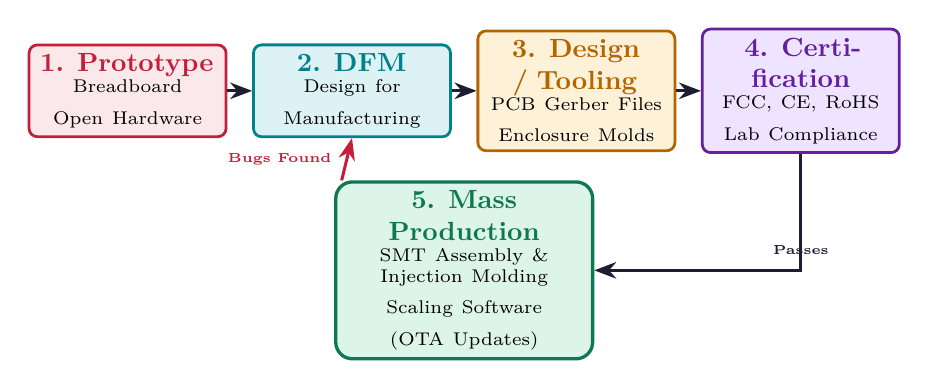
\begin{tikzpicture}[scale=0.95, transform shape]
  % Nodes
  \node[draw=myred, fill=hdrred, rounded corners=3pt, line width=1pt, text width=2.4cm, align=center, minimum height=1.1cm] (proto) at (-4.5, 0) {
    \textbf{\color{myred}1. Prototype}\\
    \scriptsize Breadboard\\
    \scriptsize Open Hardware
  };

  \node[draw=myteal, fill=hdrteal, rounded corners=3pt, line width=1pt, text width=2.4cm, align=center, minimum height=1.1cm] (dfm) at (-1.5, 0) {
    \textbf{\color{myteal}2. DFM}\\
    \scriptsize Design for\\
    \scriptsize Manufacturing
  };

  \node[draw=myamber, fill=hdramber, rounded corners=3pt, line width=1pt, text width=2.4cm, align=center, minimum height=1.1cm] (tool) at (1.5, 0) {
    \textbf{\color{myamber}3. Design / Tooling}\\
    \scriptsize PCB Gerber Files\\
    \scriptsize Enclosure Molds
  };

  \node[draw=mypurple, fill=hdrpurple, rounded corners=3pt, line width=1pt, text width=2.4cm, align=center, minimum height=1.1cm] (cert) at (4.5, 0) {
    \textbf{\color{mypurple}4. Certification}\\
    \scriptsize FCC, CE, RoHS\\
    \scriptsize Lab Compliance
  };

  \node[draw=mygreen, fill=hdrgreen, rounded corners=6pt, line width=1.2pt, text width=3.2cm, align=center, minimum height=1.2cm] (prod) at (0, -2.4) {
    \textbf{\color{mygreen}5. Mass Production}\\
    \scriptsize SMT Assembly \& Injection Molding\\
    \scriptsize Scaling Software (OTA Updates)
  };

  % Connections
  \draw[arrow, line width=1.1pt] (proto) -- (dfm);
  \draw[arrow, line width=1.1pt] (dfm) -- (tool);
  \draw[arrow, line width=1.1pt] (tool) -- (cert);
  
  % Passes arrow - enters prod.east horizontally from the right to avoid border-riding
  \draw[arrow, line width=1.1pt] (cert.south) |- node[midway, above=2pt, font=\tiny\bfseries] {Passes} (prod.east);
    
  % Bugs Found feedback loop - clean straight vertical line to dfm.south
  \draw[arrow, line width=1.1pt, color=myred] ($(prod.north west)+(0.1, 0)$) -- node[midway, left=2pt, font=\tiny\bfseries] {Bugs Found} (dfm.south);
\end{tikzpicture}
\end{tcolorbox}

\subsection{Designing and Manufacturing PCBs}
\begin{enumerate}[leftmargin=*, itemsep=4.0pt]
  \item \textbf{Schematic Capture:} Drawing the logical connectivity diagram between components using CAD software (e.g. KiCad, Altium).
  \item \textbf{PCB Layout Routing:} Arranging physical component footprints and routing copper traces to connect pins. Features include:
        \begin{itemize}[leftmargin=*, label=$\bullet$, itemsep=1.0pt]
          \item \textit{Trace Width:} Thicker traces are routed for power lines to handle current without overheating; thin traces are used for signals.
          \item \textit{Vias:} Plated copper cylinders that bridge traces between different layer planes.
          \item \textit{Ground Planes:} Large copper planes added to shield signals from EMI and provide a stable reference voltage.
        \end{itemize}
  \item \textbf{PCB Fabrication Steps:}
        \begin{itemize}[leftmargin=*, label=$\bullet$, itemsep=1.0pt]
          \item \textit{Etching:} Removing unwanted copper from substrate using chemical etchants (e.g. Ferric Chloride or Ammonium Persulfate).
          \item \textit{Drilling \& Electroplating:} Drilling mounting and via holes, then electroplating them with copper to establish layer connections.
          \item \textit{Solder Mask:} Applying a polymer layer (usually green) to insulate copper traces and prevent solder bridging.
          \item \textit{Surface Finish:} Coating exposed copper pads to prevent oxidation (e.g. \textbf{HASL} - Hot Air Solder Leveling, cheap; or \textbf{ENIG} - Electroless Nickel Immersion Gold, high-quality flat pads for fine SMT components).
        \end{itemize}
  \item \textbf{Assembly (SMT vs. Through-Hole):}
        \begin{itemize}[leftmargin=*, label=$\bullet$, itemsep=1pt]
          \item \textbf{SMT (Surface Mount Technology):} Components (SMD) are placed on solder paste and reflowed in an oven. Automated via pick-and-place machines; allows dual-sided, high-density designs.
          \item \textbf{Through-Hole Technology (THT):} Component pins are inserted through holes and wave-soldered. Essential for connectors and heavy power modules due to high mechanical strength.
        \end{itemize}
\end{enumerate}

\subsection{Mass-Producing Enclosures (Injection Molding)}
\begin{tcolorbox}[defbox, title={Injection Molding}]
  \textbf{Injection Molding} is the primary manufacturing process for plastic enclosures. Molten plastic (ABS, Polycarbonate) is injected under high pressure into a custom-machined steel or aluminum mold cavity, where it cools and solidifies into the final case.
\end{tcolorbox}
Key design constraints and manufacturing parameters for injection-molded parts:
\begin{itemize}[leftmargin=*, itemsep=3.0pt]
  \item \textbf{High Tooling Costs:} Machining the steel molds (tooling) is extremely expensive (often $\$10,000$ to $\$100,000$ NRE costs), requiring massive production volumes to amortize the setup cost.
  \item \textbf{Draft Angles:} Vertical walls must be tapered slightly (typically $1^\circ$ to $2^\circ$) to allow the solidified plastic part to eject easily from the steel mold without scratching.
  \item \textbf{Common Molding Defects:}
        \begin{itemize}[leftmargin=*, label=$\bullet$, itemsep=1.5pt]
          \item \textit{Sink Marks:} Shallow depressions formed on thick wall sections due to slower cooling and volumetric shrinkage. Fixed by maintaining uniform wall thickness.
          \item \textit{Warping:} Distortion of flat surfaces caused by non-uniform cooling rates across different sections of the part.
          \item \textit{Knit Lines (Weld Lines):} Lines where multiple molten plastic flow fronts meet and fail to fuse completely, representing structural weak spots.
          \item \textit{Flash:} Excess plastic leakage that escapes along the parting line of the mold halves due to low clamping pressure.
        \end{itemize}
\end{itemize}

\subsection{Hardware Certification}
Before selling electronic products, they must satisfy regulatory standards:
\begin{itemize}[leftmargin=*, itemsep=3.5pt]
  \item \textbf{FCC (Federal Communications Commission) Certification:} Required for products sold in the United States. It regulates electromagnetic compatibility (EMC):
        \begin{itemize}[leftmargin=*, label=$\bullet$, itemsep=1.0pt]
          \item \textit{Intentional Radiators:} Devices that actively broadcast RF signals (e.g. Wi-Fi, Bluetooth, cellular). Require full, expensive transmitter testing and registration.
          \item \textit{Unintentional Radiators:} Devices that do not intentionally broadcast radio signals but generate internal high-frequency signals ($>9\text{ kHz}$) like CPU clocks. Require self-declaration or verification.
        \end{itemize}
  \item \textbf{CE (Conformité Européenne) Marking:} Mandatory for products in the European Economic Area. Declares that the product complies with health, safety, and environmental protection directives (such as the Radio Equipment Directive - RED, and EMC Directive).
  \item \textbf{RoHS (Restriction of Hazardous Substances):} Restricts the use of specific hazardous substances in electrical and electronic equipment (specifically Lead, Mercury, Cadmium, Hexavalent Chromium, and flame retardants like PBB/PBDE). Requires lead-free solder and components.
\end{itemize}

\subsection{Manufacturing Cost Concepts}
Managing economics is critical when moving to mass manufacture:
\begin{itemize}[leftmargin=*, itemsep=3.5pt]
  \item \textbf{BOM (Bill of Materials):} A complete, hierarchical spreadsheet list of every raw component, IC, circuit board, enclosure part, connector, screw, and label required to manufacture one single unit, including supplier part numbers and cost-breaks.
  \item \textbf{NRE (Non-Recurring Engineering):} The one-time, upfront development cost of design, PCB routing labor, test fixture setup, compliance testing, and steel injection molds.
\end{itemize}
\begin{tcolorbox}[formulabox, title={Amortized Unit Cost Formula}]
  The total per-unit production cost ($U$) for a manufacturing run of $N$ units is:
  \begin{equation}
    U = \text{BOM} + \frac{\text{NRE}}{N}
  \end{equation}
  As $N \rightarrow \infty$, the amortized cost approaches the BOM cost. Small runs (low $N$) have high per-unit costs due to the unamortized NRE.
\end{tcolorbox}

\subsection{Software Scaling and OTA Updates}
When scaling from 1 to 10,000 devices:
\begin{itemize}[leftmargin=*, itemsep=2pt]
  \item Devices must support \textbf{OTA (Over-the-Air) Firmware Updates} to patch security bugs remotely over Wi-Fi/cellular without physical access.
\end{itemize}

% ===============================================================================
\section{Ethics, Security \& Environmental Solutions}
% ===============================================================================

Connecting billions of physical devices introduces deep social and environmental challenges.

\subsection{Characterizing the Internet of Things (Ethical Perspective)}
The ethical challenges of IoT are characterized by three core traits:
\begin{itemize}[leftmargin=*, itemsep=3.0pt]
  \item \textbf{Pervasiveness (Ubiquity):} Devices are embedded in private spaces (homes, offices, bodies) and gather data continuously and invisibly, leaving users unaware of the data collection.
  \item \textbf{Physical Agency:} Unlike the traditional internet (which only displays information), IoT has physical actuators that control real-world environments. A breach can cause immediate physical danger (e.g., unlocking a smart door or disabling a smart brake).
  \item \textbf{Data Ownership and Asymmetry:} A massive imbalance exists between the user (who generates the data) and the manufacturer/service provider (who aggregates, analyzes, and often sells the data).
\end{itemize}

\subsection{Privacy and Control}
IoT devices gather intimate details (voices, camera feeds, occupancy).
\begin{itemize}[leftmargin=*, itemsep=2.5pt]
  \item \textbf{Security:} Many IoT devices have weak security (default passwords, unencrypted firmware). Attackers can hijack them to form \textbf{Botnets} (e.g. Mirai botnet) to launch DDoS attacks on servers.
  \item \textbf{Control:} Who owns the data collected by a smart thermostat? Device makers must ensure localized user consent and encrypt data during transmission (using SSL/TLS or DTLS).
\end{itemize}

\subsection{Environmental Impact (E-Waste)}
\begin{itemize}[leftmargin=*, itemsep=3pt]
  \item Millions of short-lived IoT tags and smart devices end up in landfills, leading to heavy metal (lead, mercury) contamination in soil.
  \item \textbf{Solutions:} Designing for repairability, using modular component slots, and using biodegradable paper substrates or organic components for temporary IoT sensors.
\end{itemize}

\newpage

% ═══════════════════════════════════════════════════════════════════════════════
% QUICK REVISION PAGE
% ═══════════════════════════════════════════════════════════════════════════════
\begin{center}
  {\large\bfseries\color{myred} Quick Revision — Module 6}\\[3pt]
  {\small\color{mydark} Prototype to Reality $|$ OE-EC803A}
\end{center}
\noindent{\color{myred}\rule{\linewidth}{1.2pt}}
\vspace{8pt}

\begin{tcolorbox}[formulabox, title={\textbf{Key Cost and Amortization Formulas}}]
\renewcommand{\arraystretch}{1.35}
\begin{tabularx}{\linewidth}{B{5.0cm} X}
  Total Unit Cost & $\text{Cost}_{\text{unit}} = \text{BOM Cost} + \text{Assembly Cost} + \dfrac{\text{NRE Cost}}{N}$ \\[4pt]
  BOM Cost & $\text{BOM} = \sum (\text{Component Cost}_i \times \text{Quantity}_i) \quad (\text{list of materials})$ \\[4pt]
  NRE Costs & Amortized over production run volume $N$. High volume shrinks NRE impact.
\end{tabularx}
\end{tcolorbox}

\vspace{6pt}

\begin{tcolorbox}[defbox, title={\textbf{One-Line Definitions}}]
\begin{itemize}[leftmargin=*, itemsep=3pt, topsep=0pt]
  \item \textbf{Gerber File:} Standard file format containing physical layer instructions for manufacturing PCBs.
  \item \textbf{SMT:} Automated technology where electronic components are mounted directly onto the surface of a PCB.
  \item \textbf{Draft Angle:} A slight taper (1-2 degrees) on vertical walls of a molded case to allow easy ejection.
  \item \textbf{RoHS:} A directive restricting hazardous lead, mercury, and cadmium in electronic components.
  \item \textbf{OTA Update:} The process of upgrading a device's firmware wirelessly over the network.
\end{itemize}
\end{tcolorbox}

\vspace{6pt}

\begin{tcolorbox}[exambox, title={\textbf{Frequently Asked / Viva Questions}}]
\begin{enumerate}[leftmargin=*, topsep=0pt, label=\textbf{Q\arabic*.}, itemsep=6pt]
  \item \Q{What is a Gerber file, and why is it important in PCB manufacturing?}
        A Gerber file is a set of open 2D vector images showing the copper traces, solder masks, silkscreen labels, and drill paths for each layer of the PCB. PCB fabrication houses require Gerber files to program their automated drilling and etching machines.
        
  \item \Q{What is the difference between SMT and Through-Hole assembly?}
        SMT (Surface Mount) components are soldered directly to pad surfaces on the board, allowing automated high-density assembly. Through-Hole components have long wire leads inserted through holes in the board and soldered on the opposite side, which provides superior mechanical strength for heavy components like terminals and power relays.
        
  \item \Q{Why are upfront tooling costs for plastic injection molding extremely high?}
        The molds must be custom-machined out of solid blocks of hardened tool steel using high-precision CNC machines to withstand thousands of high-pressure, high-temperature plastic injection cycles. This setup cost (NRE) is high but reduces the cost per part to cents at high volumes.
        
  \item \Q{What is a draft angle in injection molding, and why is it required?}
        A draft angle is a slight taper (typically $1^\circ$ to $2^\circ$) added to the vertical walls of the plastic enclosure design. Without this taper, the cooling plastic shrinks slightly around the mold cavities, causing high friction and damage during ejection.
        
  \item \Q{Explain the role of FCC certification for IoT devices.}
        The FCC (Federal Communications Commission) regulates RF emissions. Any digital device switching signals at high speeds or using wireless transmitters must undergo testing to prove it does not emit electromagnetic interference (EMI) that could disrupt other communications.
        
  \item \Q{What is a Bill of Materials (BOM) in hardware manufacturing?}
        A BOM is a structured table listing every single component, PCB substrate, connector, case, fastener, label, and packaging box required to manufacture a single product, along with manufacturer part numbers and costs.
        
  \item \Q{How can IoT devices pose a security threat to other internet services?}
        Many consumer IoT devices lack secure firewalls and default login credentials. Attackers can scan the web and infect thousands of these vulnerable devices with malware, forming a botnet (such as Mirai) to launch massive Distributed Denial of Service (DDoS) attacks.
        
  \item \Q{What is the Product-as-a-Service (PaaS) business model in IoT?}
        In PaaS, rather than paying a large one-time fee to own hardware, customers buy hardware cheaply and subscribe to a service (recurring revenue stream). The value is delivered through ongoing cloud monitoring, alerts, and automatic software updates.
\end{enumerate}
\end{tcolorbox}

\vspace{6pt}

\begin{tcolorbox}[tikzbox, title={\textbf{Comparison Snapshot}}]
\textbf{3D Printing vs. Injection Molding for Enclosure Production:}\par\vspace{6pt}\noindent
{\renewcommand{\arraystretch}{1.35}%
\begin{tabularx}{\linewidth}{|B{3.2cm}|Y|Y|}
\hline
\textbf{Feature} & \textbf{3D Printing (Prototype)} & \textbf{Injection Molding (Mass Production)} \\
\hline
Upfront Tooling Cost & Zero (direct print from STL). & Extremely High ($\$10,000+$ for steel molds). \\
\hline
Unit Cost & Medium-High (PLA filament cost per hour). & Extremely Low (cents per plastic part). \\
\hline
Production Cycle Time & Slow (several hours per enclosure). & Very Fast (seconds per enclosure injection). \\
\hline
Design Constraints & Layer lines, support structures needed. & Draft angles, uniform wall thickness required. \\
\hline
Best Volume & 1 to 50 units (prototypes). & $5,000+$ units (mass market). \\
\hline
\end{tabularx}}
\end{tcolorbox}

\end{document}
